\documentclass{article}

\begin{document}
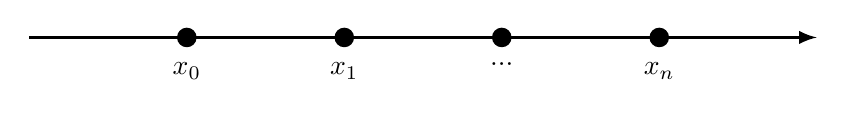
\begin{tikzpicture}
		\newcommand*{\dotSize}{2.5pt}
		\newcommand*{\belowLabel}{2mm}

		\coordinate(A) at	(0,0);
		\coordinate(B) at	(10,0);
		\coordinate(X0) at	(2,0);
		\coordinate(X1) at	(4,0);
		\coordinate(Xm) at	(6,0);
		\coordinate(Xn) at	(8,0);

		\draw[-latex, very thick] (A) -- (B);

		\node at (X0)[circle,fill,inner sep=\dotSize]{};
		\node at (X1)[circle,fill,inner sep=\dotSize]{};
		\node at (Xm)[circle,fill,inner sep=\dotSize]{};
		\node at (Xn)[circle,fill,inner sep=\dotSize]{};

		\node[below=\belowLabel] at (X0) {$x_0$};
		\node[below=\belowLabel] at (X1) {$x_1$};
		\node[below=\belowLabel] at (Xm) {$...$};
		\node[below=\belowLabel] at (Xn) {$x_n$};
\end{tikzpicture}
\end{document}